\chapter{The Forking Path: Control Flow \& Logic}

\begin{figure}[h!]
    \centering
    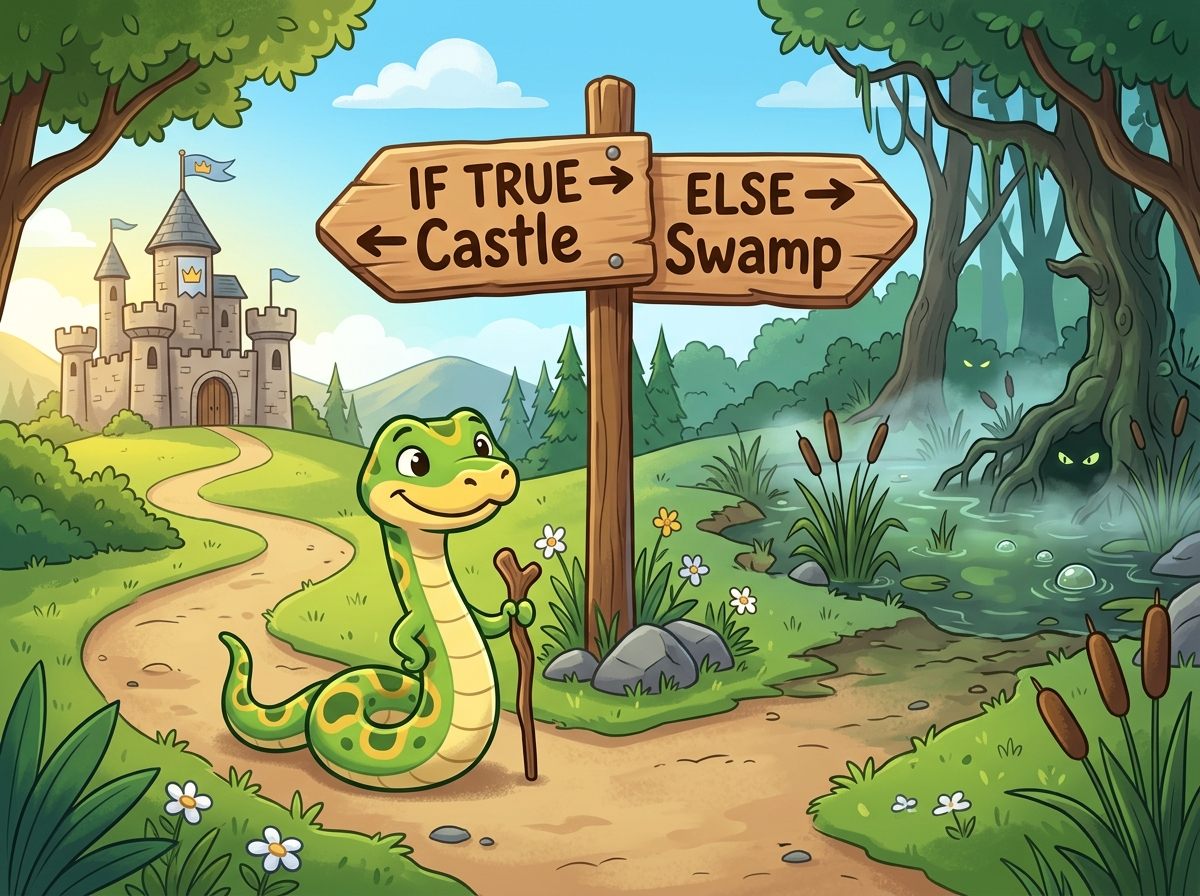
\includegraphics[width=0.75\textwidth]{images/ch2_crossroads.jpg}
    \caption{Control flow lets your code make choices like choosing a path at a crossroad.}
\end{figure}

\section{Life is Full of Choices... and So is Code!}

Without decisions, a program would just run top-to-bottom like a train on a single track. But real life requires choices: \textit{If} it rains, take an umbrella; \textit{else}, wear sunglasses!

In Python, we direct the flow of execution using \textbf{conditional statements}: \texttt{if}, \texttt{elif} (short for else-if), and \texttt{else}.

\section{The Honest Truth: Booleans \& Comparison Operators}

Before making decisions, Python evaluates questions to find if they are \texttt{True} or \texttt{False}. We ask questions using comparison operators:

\begin{table}[h!]
\centering
\begin{tabular}{|c|l|c|}
\hline
\rowcolor{pyblue!20} \textbf{Operator} & \textbf{Meaning} & \textbf{Example ($5$ vs $10$)} \\ \hline
\texttt{==} & Equals (Are they identical?) & \texttt{5 == 10} $\rightarrow$ \texttt{False} \\ \hline
\texttt{!=} & Not Equals (Are they different?) & \texttt{5 != 10} $\rightarrow$ \texttt{True} \\ \hline
\texttt{>} & Greater Than & \texttt{5 > 10} $\rightarrow$ \texttt{False} \\ \hline
\texttt{<} & Less Than & \texttt{5 < 10} $\rightarrow$ \texttt{True} \\ \hline
\texttt{>=} & Greater Than or Equal To & \texttt{5 >= 5} $\rightarrow$ \texttt{True} \\ \hline
\texttt{<=} & Less Than or Equal To & \texttt{10 <= 5} $\rightarrow$ \texttt{False} \\ \hline
\end{tabular}
\caption{Python Comparison Operators}
\end{table}

\begin{viperpitfall}{The Single vs Double Equals Trap!}
Single equals (\texttt{=}) is for \textbf{assignment} (putting stuff in a container).
Double equals (\texttt{==}) is for \textbf{comparison} (asking if two things match).
If you write \texttt{if age = 18:}, Python will throw a syntax error and scold you!
\end{viperpitfall}

\section{The Choose-Your-Own-Adventure Branch}

Here is how you write a basic conditional block in Python:

\begin{pycode}{If-Elif-Else in Action}
dragon_hunger_level = 85

if dragon_hunger_level > 90:
    print("RUN FOR YOUR LIFE! The dragon wants to eat you!")
elif dragon_hunger_level > 50:
    print("Toss a marshmallow to buy yourself 10 seconds.")
else:
    print("The dragon is sleeping peacefully. You may pass.")
\end{pycode}

\section{Logical Operators: Combining Questions}

Sometimes you need to check multiple conditions at once:
\begin{itemize}
    \item \textbf{\texttt{and}:} Returns \texttt{True} ONLY if BOTH conditions are True.
    \item \textbf{\texttt{or}:} Returns \texttt{True} if AT LEAST ONE condition is True.
    \item \textbf{\texttt{not}:} Flips the boolean value (\texttt{True} becomes \texttt{False}).
\end{itemize}

\begin{pycode}{Combining Logic}
has_key = True
knows_password = False
is_admin = True

# Door opening logic
if (has_key and knows_password) or is_admin:
    print("ACCESS GRANTED! Welcome to the secret lair.")
else:
    print("ACCESS DENIED! The alarm is ringing!")
\end{pycode}

\section{Code Example: Theme Park Ticket Tier Classifier}

Let's examine how real-world nested conditions classify theme park admission ticket prices based on visitor age and height requirements.

\begin{pycode}{Theme Park Ticket Pricing}
visitor_age = 14
height_cm = 155
is_weekend = True

# Base pricing tiers
if visitor_age < 5:
    ticket_price = 0.00
    category = "Toddler (Free)"
elif visitor_age <= 17:
    ticket_price = 15.00
    category = "Youth"
else:
    ticket_price = 25.00
    category = "Adult"

# Weekend surcharge
if is_weekend and ticket_price > 0:
    ticket_price += 5.00

# Height check for rollercoaster
can_ride_rollercoaster = height_cm >= 140

print(f"Ticket Category: {category}")
print(f"Final Ticket Price: ${ticket_price:.2f}")
print(f"Rollercoaster Eligible: {can_ride_rollercoaster}")
\end{pycode}

\begin{snakesnack}{Indentation Rule}
Always use 4 spaces per indentation level. Do not mix tabs and spaces in the same file unless you want to trigger Python's infamous \texttt{IndentationError}!
\end{snakesnack}

\section{Practice Problems \& Exercises}

Put your decision-making skills to the test with these 3 logic exercises!

\begin{snakelab}{Problem 2.1: The Magic Bouncer (Easy)}
Write a program with variables \texttt{age = 19} and \texttt{is\_vip = False}.
\begin{itemize}
    \item If age is 21 or older, OR if \texttt{is\_vip} is True, print ``Welcome to the Python Lounge!''
    \item Otherwise, print ``Entry denied! Come back when you're older.''
\end{itemize}
\end{snakelab}

\begin{pycode}{Solution 2.1: Magic Bouncer}
age = 19
is_vip = False

if age >= 21 or is_vip:
    print("Welcome to the Python Lounge!")
else:
    print("Entry denied! Come back when you're older.")
\end{pycode}

\begin{snakelab}{Problem 2.2: Leap Year Detector (Medium)}
A year is a leap year if it is divisible by $4$, EXCEPT if it is divisible by $100$, UNLESS it is also divisible by $400$.
Write a script testing \texttt{year = 2024} and \texttt{year = 1900} to print whether each year is a leap year!
\end{snakelab}

\begin{pycode}{Solution 2.2: Leap Year Detector}
year = 2024

if (year % 4 == 0 and year % 100 != 0) or (year % 400 == 0):
    print(f"Year {year} is a LEAP YEAR!")
else:
    print(f"Year {year} is a standard year.")
\end{pycode}

\begin{snakelab}{Problem 2.3: RPG Critical Hit Calculator (Spicy)}
Given a player's attack power of $50$ and a random dice roll value between $1$ and $20$:
\begin{itemize}
    \item If dice roll is $20$: Critical hit! Multiply damage by $3$.
    \item If dice roll is $15$ to $19$: Strong hit! Multiply damage by $1.5$.
    \item If dice roll is $2$ to $14$: Normal hit! Deal base damage ($50$).
    \item If dice roll is $1$: Critical fumble! Deal $0$ damage and print a clumsy message.
\end{itemize}
\end{snakelab}

\begin{pycode}{Solution 2.3: Critical Hit Calculator}
base_attack = 50
dice_roll = 20  # Simulated roll

if dice_roll == 20:
    damage = base_attack * 3
    print(f"NAT 20! CRITICAL HIT! Dealt {damage} damage!")
elif dice_roll >= 15:
    damage = base_attack * 1.5
    print(f"Great hit! Dealt {damage:.0f} damage.")
elif dice_roll >= 2:
    damage = base_attack
    print(f"Normal hit. Dealt {damage} damage.")
else:
    damage = 0
    print("CRITICAL FUMBLE! You tripped over your own cape and dealt 0 damage!")
\end{pycode}
